\documentclass[twoside]{book}

% Packages required by doxygen
\usepackage{fixltx2e}
\usepackage{calc}
\usepackage{doxygen}
\usepackage[export]{adjustbox} % also loads graphicx
\usepackage{graphicx}
\usepackage[utf8]{inputenc}
\usepackage{makeidx}
\usepackage{multicol}
\usepackage{multirow}
\PassOptionsToPackage{warn}{textcomp}
\usepackage{textcomp}
\usepackage[nointegrals]{wasysym}
\usepackage[table]{xcolor}

% Font selection
\usepackage[T1]{fontenc}
\usepackage[scaled=.90]{helvet}
\usepackage{courier}
\usepackage{amssymb}
\usepackage{sectsty}
\renewcommand{\familydefault}{\sfdefault}
\allsectionsfont{%
  \fontseries{bc}\selectfont%
  \color{darkgray}%
}
\renewcommand{\DoxyLabelFont}{%
  \fontseries{bc}\selectfont%
  \color{darkgray}%
}
\newcommand{\+}{\discretionary{\mbox{\scriptsize$\hookleftarrow$}}{}{}}

% Page & text layout
\usepackage{geometry}
\geometry{%
  a4paper,%
  top=2.5cm,%
  bottom=2.5cm,%
  left=2.5cm,%
  right=2.5cm%
}
\tolerance=750
\hfuzz=15pt
\hbadness=750
\setlength{\emergencystretch}{15pt}
\setlength{\parindent}{0cm}
\setlength{\parskip}{3ex plus 2ex minus 2ex}
\makeatletter
\renewcommand{\paragraph}{%
  \@startsection{paragraph}{4}{0ex}{-1.0ex}{1.0ex}{%
    \normalfont\normalsize\bfseries\SS@parafont%
  }%
}
\renewcommand{\subparagraph}{%
  \@startsection{subparagraph}{5}{0ex}{-1.0ex}{1.0ex}{%
    \normalfont\normalsize\bfseries\SS@subparafont%
  }%
}
\makeatother

% Headers & footers
\usepackage{fancyhdr}
\pagestyle{fancyplain}
\fancyhead[LE]{\fancyplain{}{\bfseries\thepage}}
\fancyhead[CE]{\fancyplain{}{}}
\fancyhead[RE]{\fancyplain{}{\bfseries\leftmark}}
\fancyhead[LO]{\fancyplain{}{\bfseries\rightmark}}
\fancyhead[CO]{\fancyplain{}{}}
\fancyhead[RO]{\fancyplain{}{\bfseries\thepage}}
\fancyfoot[LE]{\fancyplain{}{}}
\fancyfoot[CE]{\fancyplain{}{}}
\fancyfoot[RE]{\fancyplain{}{\bfseries\scriptsize Generated by Doxygen }}
\fancyfoot[LO]{\fancyplain{}{\bfseries\scriptsize Generated by Doxygen }}
\fancyfoot[CO]{\fancyplain{}{}}
\fancyfoot[RO]{\fancyplain{}{}}
\renewcommand{\footrulewidth}{0.4pt}
\renewcommand{\chaptermark}[1]{%
  \markboth{#1}{}%
}
\renewcommand{\sectionmark}[1]{%
  \markright{\thesection\ #1}%
}

% Indices & bibliography
\usepackage{natbib}
\usepackage[titles]{tocloft}
\setcounter{tocdepth}{3}
\setcounter{secnumdepth}{5}
\makeindex

% Hyperlinks (required, but should be loaded last)
\usepackage{ifpdf}
\ifpdf
  \usepackage[pdftex,pagebackref=true]{hyperref}
\else
  \usepackage[ps2pdf,pagebackref=true]{hyperref}
\fi
\hypersetup{%
  colorlinks=true,%
  linkcolor=blue,%
  citecolor=blue,%
  unicode%
}

% Custom commands
\newcommand{\clearemptydoublepage}{%
  \newpage{\pagestyle{empty}\cleardoublepage}%
}

\usepackage{caption}
\captionsetup{labelsep=space,justification=centering,font={bf},singlelinecheck=off,skip=4pt,position=top}

%===== C O N T E N T S =====

\begin{document}

% Titlepage & ToC
\hypersetup{pageanchor=false,
             bookmarksnumbered=true,
             pdfencoding=unicode
            }
\pagenumbering{roman}
\begin{titlepage}
\vspace*{7cm}
\begin{center}%
{\Large My Project }\\
\vspace*{1cm}
{\large Generated by Doxygen 1.8.11}\\
\end{center}
\end{titlepage}
\clearemptydoublepage
\tableofcontents
\clearemptydoublepage
\pagenumbering{arabic}
\hypersetup{pageanchor=true}

%--- Begin generated contents ---
\chapter{File Index}
\section{File List}
Here is a list of all documented files with brief descriptions\+:\begin{DoxyCompactList}
\item\contentsline{section}{/home/vinit/workspace/c++/\+My\+First\+Project/mylib/{\bfseries sum.\+hpp} }{\pageref{sum_8hpp}}{}
\item\contentsline{section}{/home/vinit/workspace/c++/\+My\+First\+Project/mylib/\hyperlink{version_8hpp}{version.\+hpp} \\*My\+First\+Project configuration file }{\pageref{version_8hpp}}{}
\end{DoxyCompactList}

\chapter{File Documentation}
\hypertarget{version_8hpp}{}\section{/home/vinit/workspace/c++/\+My\+First\+Project/mylib/version.hpp File Reference}
\label{version_8hpp}\index{/home/vinit/workspace/c++/\+My\+First\+Project/mylib/version.\+hpp@{/home/vinit/workspace/c++/\+My\+First\+Project/mylib/version.\+hpp}}


My\+First\+Project configuration file.  


This graph shows which files directly or indirectly include this file\+:
\nopagebreak
\begin{figure}[H]
\begin{center}
\leavevmode
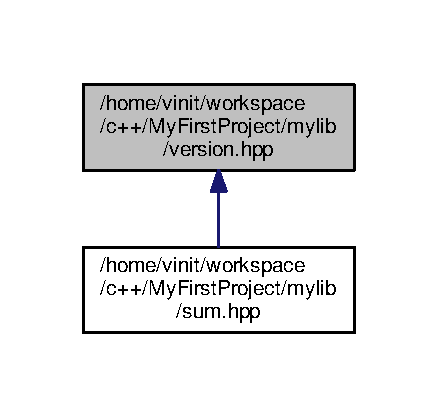
\includegraphics[width=210pt]{version_8hpp__dep__incl}
\end{center}
\end{figure}
\subsection*{Macros}
\begin{DoxyCompactItemize}
\item 
\#define {\bfseries My\+First\+Project\+\_\+\+V\+E\+R\+S\+I\+O\+N\+\_\+\+M\+A\+J\+OR}~1\hypertarget{version_8hpp_a8f08c0f5438003ad202db2c4fe81b185}{}\label{version_8hpp_a8f08c0f5438003ad202db2c4fe81b185}

\item 
\#define {\bfseries My\+First\+Project\+\_\+\+V\+E\+R\+S\+I\+O\+N\+\_\+\+M\+I\+N\+OR}~0\hypertarget{version_8hpp_a3690a569dd90cd5eef87ffa0e97354e9}{}\label{version_8hpp_a3690a569dd90cd5eef87ffa0e97354e9}

\item 
\#define {\bfseries My\+First\+Project\+\_\+\+V\+E\+R\+S\+I\+O\+N\+\_\+\+P\+A\+T\+CH}~0\hypertarget{version_8hpp_a6deb22355edbd65b5c856b07f28cb0ab}{}\label{version_8hpp_a6deb22355edbd65b5c856b07f28cb0ab}

\item 
\#define {\bfseries My\+First\+Project\+\_\+\+G\+I\+T\+\_\+\+R\+E\+V\+I\+S\+I\+ON}~\char`\"{}\char`\"{}\hypertarget{version_8hpp_a0bb55bca0a046319e7b5a70db1e31e8b}{}\label{version_8hpp_a0bb55bca0a046319e7b5a70db1e31e8b}

\item 
\#define {\bfseries My\+First\+Project\+\_\+\+S\+Y\+S\+T\+E\+M\+\_\+\+N\+A\+ME}~Linux\hypertarget{version_8hpp_a343e81fc018fa54b7b91fc92c574b065}{}\label{version_8hpp_a343e81fc018fa54b7b91fc92c574b065}

\item 
\#define {\bfseries My\+First\+Project\+\_\+\+H\+O\+S\+T\+\_\+\+S\+Y\+S\+T\+E\+M\+\_\+\+P\+R\+O\+C\+E\+S\+S\+OR}~x86\+\_\+64\hypertarget{version_8hpp_aebf433fc920c03f9366016d055e3fffd}{}\label{version_8hpp_aebf433fc920c03f9366016d055e3fffd}

\end{DoxyCompactItemize}


\subsection{Detailed Description}
My\+First\+Project configuration file. 

\begin{DoxyAttention}{Attention}
automatically generated from {\bfseries config.\+hpp.\+in}, do not modify! 
\end{DoxyAttention}

%--- End generated contents ---

% Index
\backmatter
\newpage
\phantomsection
\clearemptydoublepage
\addcontentsline{toc}{chapter}{Index}
\printindex

\end{document}
